\documentclass[a4paper,12pt]{article}
\usepackage[utf8]{inputenc}
\usepackage{graphicx}
\usepackage{cite}

\graphicspath{{}}

\title{Research Plan Force-directed Graph Drawing}
\author{
  Michiel van Heusden, 4173309 \and
  Maurits van der Veen, 4167287 \and
  Kevin Oosterlaak, 4012372 \and
  Jesse Ceelen, 4061837
  }
\date{\today}

\begin{document}
  \maketitle
  \tableofcontents
  \section{intro}
  Data requires often visualization before people understand what it means.
  This visualization is done with graphs and charts.
  This research focuses on the drawing methods of graphs.
  These graphs consist of objects and the relations between them.
  In graph theory the objects are called vertices and their relations edges.\cite{bondy1976graph}
  Generating readable graphs becomes more difficult as the amount of vertices and edges grows.
  To generate these correctly many algorithms were developed.
  One family of algorithms to do this is called \emph{Force Directed Graph Drawing}.
  The idea behind force directed graph drawing is to treat the graph as a physical system and iterate on the forces acting on it until the result stabilizes. In this research several of these algorithms will be tested and compared to see which generates the most readable graphs.
  Not only will we compare different algorithms, we will also look at how the parameters of these algorithms affect the results.

  \subsection{The Algorithms}\label{par:algorithms}
    The method used for each of the tests is the same,  except for the way the forces are calculated.
    Said method is for each vertex to iterate over the other vertices and calculate the repulsive force between them.
    Then the same is done for the attractive force, but instead of iterating over vertices it iterates over all vertices connected to the current vertex by an edge. All of these forces are added together and applied to the vertex.
    
    The above is applied to every vertex, and after a sufficiently large amount of iterations the graph should have converged to a stable configuration.

    \subsubsection{Hooke-Coulomb}
    The Hooke-Coulomb algorithm is not named after its inventors, but after the laws it follows.
    The attractive forces are calculated using Hooke's Spring Law.
    The repulsive ones are based on particle physics.
    To be more precise, they are calculated using Coulomb's law of charged particles.

    Hooke's Law can be used to calculate the distance a spring extends when a certain force is applied to it.
    However, this same law can be used to calculate the required force for a spring to be extended a certain distance.
    The law itself is rather simple:
    \begin{equation}
      F = c \delta X
    \end{equation}
    Here $c$ is a constant that defines the stiffness of the spring, it is also known as te \emph{spring constant}.
    The change in length is $\delta X$, whilst $F$ is the required force.

    Coulomb's law was first published by the French physicist Charles Augustin de Coulomb in 1785.\cite{coulomb1785premier}
    Though it was first proposed for charged metal balls, it holds for charged particles.
    In his book Coulomb states for two equally electrified metal balls "\ldots the repulsive force that the two balls \ldots exert on each other, follows the inverse proportion of the square of the distance".
    This means that the repulsive force grows quadratic the closer the balls are.
    Coulomb's law can be written down as an equation as well:
    \begin{equation}
      F = k_e \frac{q_1 q_2}{r^2}
    \end{equation}
     In this equation $q_1$ and $q_2$ are the charges of the particles, $r$ is the distance between them and $k_e$ is Coulomb's Constant.\footnote{$k_e = 8.987551787 x 10^9 N m^2 C^{-2}$}

    Changing Hooke's Law to make it useful for the calculation of forces is rather straightforeward:
    Each edge corresponds to a spring, where the vertices are objects connected by springs.
    Thus we can state a rest length $l_0$ for each edge, for easy calculations we have decided on $l_0 = 1$.
    Using the ideal length -- which can be seen as the starting length of the spring -- it is possible to calculate $\delta X$:
    \begin{equation}
      \delta X =  l_d - l_0
    \end{equation}
    In this formula $l_d$ is the distance between the two connected vertices.
    The resulting formula for the attractive forces between vertices $i$ and $j$ will thus be:
    \begin{equation}
      F_a (i,j) = w_{a} (l_d - l_0) \hat{r}_{i,j}
    \end{equation}
    In this formula the constant $w_{a}$ is used instead of $c$ for future ease of distinguishing between the constants used in various formulas.
    Not only could $w_{a}$ be seen as the stiffness of the spring, it could also be seen as the weight of the attractive force, hence the new name.
    Thus it can be used to control how much influence the spring has on the vertex. $\hat{r}_{i,j}$ is the normalized vector from vector $i$ to vector $j$, calculated as $\hat{r}_{i,j} = \vec{r_{i,j}} / |\vec{r_{i,j}}|$ with $\vec{r_{i,j}}$ the vector from vertex $i$ to vertex $j$ and $|\vec{r_{i,j}}|$ the length of said vector.

    Rewriting Coulomb's law to be useful in our research requires a bit more effort.
    However, it results in the very simplified equation below.
    
    This equation is the result of some assumptions.
    First off, the charge of both the particles is assumed to be 1.
    Furthermore, since more control over the strength of this force is desired Coulomb's constant can be merged with a weight constant $w_{r}$
    \begin{equation}
      F_{r}(i,j) = w_{r} \frac{\hat{r}_{j,i}}{|\vec{r_{j,i}}|^2}
    \end{equation}
    In this equation $\hat{r}_{j,i}$ is the normalized vector from vertex $j$ to vertex $i$. This order is chosen like this to ensure that the force applied to vertex $i$ is calculated instead of the force on vertex $j$.

    \subsubsection{Fruchterman Reingold}
    The Fruchterman Reingold algorithm on the other hand is named after its inventors.\cite{fruchterman1991graph}
    For the method Fruchterman and Reingold proposed there are only two principles for graph drawing, namely that connected vertices should be drawn near each other but not \emph{too} near.
    This algorithm can be seen as being based off of the idea of ideally distributed vertices.
    It does not focus so much on each individual node as much as how far all nodes should be apart from each other.
    Like the Hooke Coulomb algorithm it is based off of particle physics:
    All vertices repel each other whilst connected vertices are attracted to each other.
    This algorithm uses a few input variables of which three will be changed:
    \begin{itemize}
	  \item Force weight $w$
      \item The optimal distance between vertices $k_{i}$
      \item The measured area $A$
    \end{itemize}
    During our testing all of these will be directly or indirectly changed.
    $w$ is the weight by which both the attractive and the repulsive forces will be scaled, directly changing their influence on the vertices.
    $k_{i}$ on the other hand will not be directly changed, but by changing constant $C$ in its formula:
    \begin{equation}\label{eq:FR_k}
      k_{i} = C \sqrt{\frac{A}{N}}
    \end{equation}
	In this equation $C$ is a constant that will be changed during testing, $A$ is the aforementioned area, circular around the vertex $i$ that $k_i$ is calculated for. This area is varied by changing its radius $r$. $N$ is then the total amount of vertices in said area, including the vertex at its center.
	
    The constant $k_{i}$ plays an important part in calculation of both the attractive and repulsive forces.
    These can be calculated using formulas \ref{eq:FR_a} and \ref{eq:FR_r} respectively.
    \begin{equation}\label{eq:FR_a}
      f_{a}(i,j) = w \frac{|\vec{r_{i,j}}|^2}{k_{i}}
    \end{equation}
    \begin{equation}\label{eq:FR_r}
      f_{r}(i,j) = - w \frac{k_{i}^2}{|\vec{r_{i,j}}|}
    \end{equation}

    Unfortunately with just these formulas the system will not converge, so a cooling function is required. The output from this cooling function acts a limit on the distance a vertex may be moved after summing all the forces applied to it. As the name suggests, this function returns a lower value every iteration, thus ensuring increasingly small changes to the graph.
    
    For our experiment a simple hyperbolic cooling function will suffice:
    \begin{equation}
	    Cooling(i) = t_{0}^{1 - \frac{i}{n}}
    \end{equation}
    Where $t_{0}$ is the initial limit, $n$ is the total amount of iterations the algorithm will run for and $i$ is the current iteration.

    \subsubsection{Eades}
    One person who has made many contributions to the research of force directed graph drawing is Peter Eades.
    This algorithm is very similar to the Hooke-Coulomb one in that it uses the same laws, with an alteration to Hooke's spring law.
    The difference between them is the type of springs used.
    The force they exert in Hooke's law grows linearly, while it grows \emph{logarithmically} in Eades' algorithm.
	This means that the more a 'spring' is extended the speed at which the force increases slows down.
    The equation for the attractive force between vertices $i$ and $j$ in Eades' algorithm is:
    \begin{equation}\label{eq:Eades_a}
      f_a(i,j) = w_{a1} log_{2}(\frac{|\vec{r_{i,j}}|}{w_{a2}})
    \end{equation}

    Aside from this changed equation the algorithm remains exactly the same.
    This formula requires two constants $w_{a1}$ and $w_{a2}$ that will be changed during testing. \cite{eades1984heuristic}

  \section{Problem Description}
    The aforementioned algorithms are meant to make graphs more readable, giving them a clear organized structure.
    Since readability is a rather vague and abstract measurement criteria in itself, there have to be concrete measurable properties that represent readability.
    The following properties can be used to express readability: \cite{kobourov2012spring}
    \begin{itemize}
      \item Uniformity of vertex distribution
      \item Uniformity of edge lengths
      \item Amount of edge crossings
    \end{itemize}
    The uniformity of vertex distribution can also be seen as the density of the vertices.
    Every vertex has an area with a fixed radius where the density can be calculated by counting the amount of vertices in that area. Division by the area is not necessary since the same area is used for all vertices, thus cancelling each other out.
    For a readable graph it is important that these densities are similar for all vertices.
    This characteristic of the uniformity of vertex distribution is then the coefficient of variation of the densities for all vertices, calculated by the standard deviation divided by the median. The lower this value, the better the graph is.

    With the uniformity of edge lengths, it is important that the lengths of all the edges are similar.
    A graph with a high variety of edge lengths is generally harder to read than a graph with edges of about equal lengths.
    This characteristic is measured with the coefficient of variation of all edge lengths. The lower this value, the better the graph is.

    For a good graph drawing, it is desirable to have as few edge crossings as possible, ideally none at all.
    Having a lot of edges that cross each other makes the graph look more chaotic and cluttered, thus making it harder to read. This characteristic is measured with the ratio of edges that cross any other edges to the total amount of edges. Again, the lower this value the better the graph is, $0$ when there are no edge crossings.

	Finally, the resulting values of these three measurements are summed to form the final Quality measure, hereafter referred to as $Q$. This $Q$ measure also indicates a better graph the smaller it is, just like its constituent components.

    Getting an as low as possible $Q$ value is what all the aforementioned algorithms strive for.
    Finding out which algorithm creates the graphs with the highest readability, which is to say the lowest $Q$ value, is what this research is meant to focus on.
    By doing these tests multiple times, we can conclude which algorithm gives the most readable graph from the results of these tests.
    Which brings us to our research question: Which force directed graph drawing algorithm yields the highest quality graphs?

  \section{The Experiment} % Beschrijving van het uitgevoerde experiment
  To conduct the experiment, a program was made that implements the three algorithms: Hooke-Coulomb, Furchterman-Reingold and Eades. There are two methods for each algorithm. A method for calculating the repulsive force between all vertices and a method for calculating the attractive force between edge-connected vertices. Each method has a parameter for the weight of the force. The methods for Fuchterman Reingold's algorithm also have a parameter for the constant C, which is used for calculating the optimal distance between vertices, and a parameter for the radius of the area around the vertex, which determines for which vertices the optimal distance is calculated. Finally, the method for calculating the attractive force in Eades' algorithm has an additional parameter for the logarithmic constant which reflects the 'stiffness' of the simulated spring. The algorithms were tested with every combination of values for the parameters. Ten different values were used for every parameter and the values were interpolated linearly. The range in which each parameter was varied is listed below:\newline
  
  \textbf{Hooke-Coulomb}
  \begin{itemize}
  	\item $w_{a}: [0.0001 \sim 0.4]$
  	\item $w_{r}: [0.0001 \sim 0.2]$
  \end{itemize}
  
  \textbf{Fuchterman Reingold}
  \begin{itemize}
  	\item $w_{a}: [0.0001 \sim 1]$
  	\item $w_{r}: [0.0001 \sim 1]$
  	\item $radius: [1 \sim 3]$
  \end{itemize}
  
  \textbf{Eades}
  \begin{itemize}
  	\item $w_{a1}: [0.0001 \sim 0.4]$
  	\item $w_{r}: [0.0001 \sim 0.2]$
  	\item $w_{a2}: [0.0001 \sim 2.0]$
  \end{itemize}
  
  In addition to these, the spring length at rest $l_{0}$ in the Hooke-Coulomb algorithm and the starting 'temperature' for the cooling schedule in the Fruchterman-Reingold algorithm were set at $0$ and $5$, respectively.
  
  The input data to test each algorithm were all graphs with 20 vertices. These graphs were randomly generated before conducting the experiment, and the same ten graphs were reused for every combination of parameter settings. Each vertex had at least one connection and could have up to 10 random connections with other vertices. The initial x and y positions of the vertices were a random double between 0 and 1. Ten of these graphs were generated and each graph was used as input for a test.
  
  Every algorithm was run for 100 iterations on each of the graphs, and each combination of parameter settings was used for every graph. After each test the quality of the output graph was measured, based on the three properties mentioned in the problem description. The average of the $Q$ values over all graphs per combination of parameters was then used as the output value in order to guarantee a t-distribution, convenient for statistical testing.

  \section{Result Data} % Eindresultaten
  Now that the tests have been conducted this section will be used to illustrate the collected data, form hypotheses and test them. Due to the expansive size of our dataset no tables or graphs have been included.
  
  %\subsection{Tabellen} % Uitgebeeld enzo
  %\subsection{Grafieken}
  %\subsection{Toelichting}
  \subsection{Statistical Hypotheses}
  Four hypotheses were tested based off of this data, three to answer our research question in detail and an additional one that arose from an observed peculiarity in collected data:
  \begin{itemize}
  	\item[1.] Hooke-Coulomb performs better than Eades
  	\item[2.] Hooke-Coulomb performs better than Fruchterman-Reingold
  	\item[3.] Eades performs worse than Fruchterman-Reingold
  	\item[4.] Changing the value of $w_{a2}$ in the Eades algorithm has a significant effect on the $Q$ value of the final graph.
  \end{itemize}
  
  The first three would be obvious to test using an independent t-test, but since the same graphs were used in all cases the data is not completely independent, making this test impossible. Instead a one-sample t-test was conducted, using the median $Q$ over all parameter configurations for the first algorithm is used as the median to compare the dataset of the other algorithm to. The function of these hypotheses should also be clear - they allow a ranking to be applied to all three algorithms indicating which one is the best, which one the second best and which one is the worst.
  
  The final hypothesis arose from an empirical observation from the data. In particular we noticed that the variations in the $w_{a2}$ constant in the Eades algorithm did not seem to affect the resulting $Q$ value much. To test this would be difficult since ten different settings of this constant were tried, but based on empirical observation of the test results we decided on a paired t-test between the lowest and the highest settings of $w_{a2}$ since they seemed to be somewhat different.
  
  So formally, the four tests are as follows, all to be conducted with a confidence of $0.95$:
  \begin{itemize}
  	\item[1.] $H_{0}: \mu_{HC} < \mu_{E}$ \\
			  $H_{1}: \mu_{HC} \geq \mu_{E}$
	\item[2.] $H_{0}: \mu_{HC} < \mu_{FR}$ \\
			  $H_{1}: \mu_{HC} \geq \mu_{FR}$
	\item[3.] $H_{0}: \mu_{E} > \mu_{FR}$ \\
		      $H_{1}: \mu_{E} \leq \mu_{FR}$
	\item[4.] $\mu_{Dw_{a2}} = \mu_{loww_{a2}} - \mu{highw_{a2}}$ \\
			  $H_{0}: \mu_{Dw_{a2}} \neq 0$ \\
			  $H_{1}: \mu_{Dw_{a2}} = 0$
  \end{itemize}
  
  Notice the directions of the inequalities - remember that a \emph{lower} $Q$ value means that the graph is better.
  
  \subsection{Hypotheses results}
  First, the Hooke-Coulomb and Eades test. The table below and all other tables thereafter were generated using IBM SPSS Statistics 23 Trial version.
  
  In this table the Test Value is the median $Q$ value of the Hooke-Coulomb data. The values in the topmost table are the statistics of the Eades data while the bottom table shows the various values resulting from the one-sample t-test. \\
  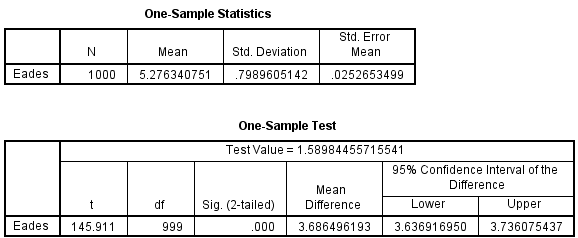
\includegraphics{HookeEadesTest}
  
  The way this table should be read is not immediately obvious, but the result is that the $Q$ values of Eades are significantly higher than those of the Hooke-Coulomb algorithm, since the t-value is much higher than $t_{crit} \approx 1.646$. So $\mu_{E} > \mu_{HC} \Rightarrow \mu_{HC} < \mu_{E}$, so the null hypothesis should not be discarded, meaning that the Hooke-Coulomb algorithm performs significantly better than the Eades algorithm. \\
  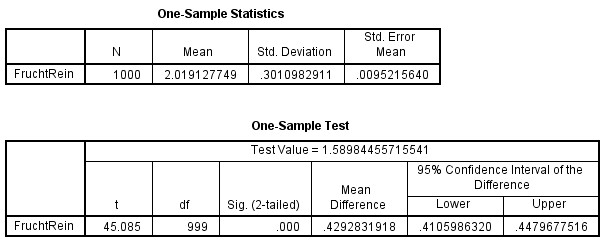
\includegraphics{HookeFRTest}
  
  This test runs parallel to the previous one. The t-value is much greater than $t_{crit} \approx 1.646$, so $\mu_{FR} > \mu_{HC} \Rightarrow \mu_{HC} < \mu_{FR}$. So the null hypothesis should not be discarded, meaning that the Hooke-Coulomb algorithm performs significantly better than the Fruchterman-Reingold algorithm. \\
  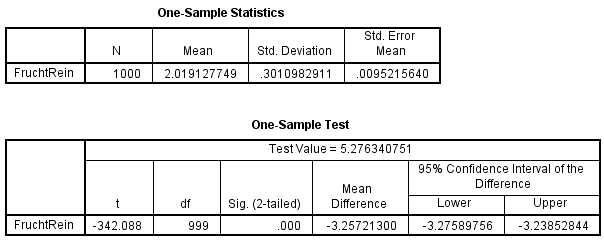
\includegraphics{EadesFRTest}
  
  Again, this works parallel to the previous two tests, with the difference that the t-value here is much lower than $-t_{crit} \approx -1.646$. So $\mu_{FR} < \mu_{E} \Rightarrow \mu_{E} > \mu_{FR}$, so the null hypothesis should not be discarded, meaning that the Eades algorithm performs significantly worse than the Fruchterman-Reingold algorithm. \\
  
  This final test reads a bit differently. The topmost table shows the statistics of both the low $w_{a2}$ and the high $w_{a2}$ values while the middle one shows the correlation between the two sample sets. The third and bottommost table shows the statistics of the difference of the two datasets as well as the test results. \\
  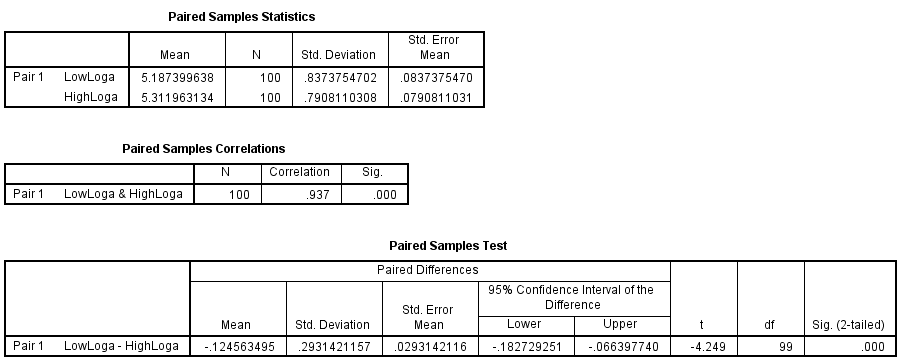
\includegraphics[width=450pt]{LogPairedTest}
  
  With 99 degrees of freedom the critical t-value is $-t_{crit} \approx -1.984$, and clearly the t-value is smaller than that, so the median of the difference between the two values is significantly different from 0. Thus the null hypothesis should not be discarded, meaning that the two values are in fact significantly different from one another. Thus varying the parameter $w_{a2}$ has a significant effect on the $Q$ values, at the very least between the highest and lowest settings. 

  \section{Conclusion \& Discussion}
  From the first three tests the result $\mu_{HK} < \mu_{FR} < \mu_{E}$ can be concluded. This means that the Hooke-Coulomb algorithm performs the best, followed by the Fruchterman-Reingold algorithm and finally by the Eades algorithm. So, at least within our testing parameters, the Hooke-Coulomb algorithm performs the best out of these three.
  
  Additionally, the $w_{a2}$ parameter in the Eades algorithm does in fact have a significant effect on the resulting $Q$ values.
  
  \section{Reflection}
  However, there are some footnotes that should be placed by these results.
  First of all, these results are not at all what we expected when we started the research. In particular, Eades' algorithm was explicitly stated to be, in general, an improvement on the Hooke-Coulomb algorithm while the opposite is true. Even more surprising is that the mean $Q$ value of the Eades algorithm is over $5$, which is not just higher than those of the Hooke-Coulomb and Fruchterman-Reingold algorithms but much higher.
  
  A possible explanation of this could be that we have been testing in a local optimum, even though we did base our testing ranges around the parameter settings that should work well according to Eades. Another possibility is that Eades' algorithm simply performs worse than Hooke-Coulomb only within the parameters the test was conducted with, while it does perform better on average, with larger graphs for example.
  
  Another strange thing is that Fruchterman-Reingold didn't perform better. Even though its performance was by no means terrible we did expect this algorithm, which is quite a bit newer than the other two algorithms, to perform better. This might be for the same reasons why the Eades algorithm performed badly.
  
  Overall, we were just not able to conduct enough meaningful tests. Being restricted to theory we were almost completely unfamiliar with and a lack of computational power and time to collect more data significantly reduced our ability to conduct proper research.
  
  For future research the optimal performance settings for each algorithm individually might be researched first, after which their results can be compared more fairly. A much wider range of graphs and parameter settings in particular would be highly desired for more accurate results.

  \bibliography{verslag}{}
  \bibliographystyle{unsrt}
\end{document}
